% !TEX program = xelatex
\documentclass[11pt,a4paper]{article}

\usepackage[margin=24mm]{geometry}
\usepackage{fontspec}
\usepackage{booktabs}
\usepackage{graphicx}
\usepackage{xcolor}
\usepackage{tikz}
\usepackage{microtype}
\usepackage{setspace}
\usepackage{caption}
\usepackage{hyperref}
\usepackage{enumitem}
\usepackage{amsmath,amssymb}
\usepackage{fancyhdr}
\usepackage{titlesec}

\setmainfont{DejaVu Serif}
\setmonofont{DejaVu Sans Mono}

\usetikzlibrary{arrows.meta,positioning}

\definecolor{Rec}{HTML}{888888}
\definecolor{APC}{HTML}{0077BB}
\definecolor{FS}{HTML}{EE7733}
\definecolor{Ink}{HTML}{1A1A1A}
\definecolor{Mute}{HTML}{5C5C5C}
\definecolor{Paper}{HTML}{F7F5F1}
\definecolor{Rule}{HTML}{D9D4CC}

\pagecolor{Paper}
\color{Ink}
\hypersetup{
  colorlinks=true,
  linkcolor=Ink,
  citecolor=Ink,
  urlcolor=APC,
  pdftitle={ForkServe: Preliminary Evaluation of Branch-Aware Serving},
}

\pagestyle{fancy}
\fancyhf{}
\fancyhead[L]{\small\color{Mute}ForkServe evaluation}
\fancyhead[R]{\small\color{Mute}Qwen3-14B $\cdot$ forest serving}
\fancyfoot[C]{\small\color{Mute}\thepage}
\renewcommand{\headrulewidth}{0.3pt}
\renewcommand{\headrule}{\hbox to\headwidth{\color{Rule}\leaders\hrule height \headrulewidth\hfill}}

\titleformat{\section}{\large\bfseries}{\thesection}{0.8em}{}
\titleformat{\subsection}{\normalsize\bfseries}{\thesubsection}{0.8em}{}
\captionsetup{font=small,labelfont={bf,color=Mute},textfont={color=Mute}}
\setlist[itemize]{leftmargin=1.4em,itemsep=0.25em}
\setstretch{1.15}

\title{\vspace{-1.8em}\textbf{ForkServe: Preliminary Evaluation of\\[-0.15em]
Branch-Aware KV Sharing against Prefix Caching}\\[0.45em]
\large Qwen3-14B forest serving --- completed runs}
\author{Dong Liu \and Chuan Wu \and contributors}
\date{GSM8K full set: 13~Sep~2026 \quad RL forest, $n{=}4$: round~3}

\begin{document}
\maketitle
\vspace{-1.2em}

\noindent
All runs, code, and logs are on host \texttt{g14} under \texttt{dliu/forkserve}.

\begin{abstract}
\noindent
On Qwen3-14B, the same Tree-of-Thoughts / ReAct forest is served by
\textbf{recompute} (vLLM, prefix cache off),
\textbf{APC} (vLLM automatic prefix caching),
and \textbf{ForkServe} (copy-on-write fork, then abort to a committed spine).

On GSM8K ($n{=}1319$, $\mathrm{tp}{=}2$), ForkServe's per-chunk peak KV is strictly below APC on $165/165$ chunks (median $1030$ vs.\ $1430$, ratio $0.72$), official accuracy is $0.845$ vs.\ $0.844$, and generate wall-clock is $18.9$ vs.\ $18.6\,\mathrm{min}$.
A $n{=}4$ forest shows the same peak ordering on GSM8K, Game24, and HumanEval at $\mathrm{tp}{=}2$, and on Game24 / HumanEval at $\mathrm{tp}{=}4$, with e2e within $2\%$ of APC.
\end{abstract}

\section{Experimental setup}

Recompute, APC, and ForkServe use the same weights, recipe, and decode budget.
Recompute prefills the full trunk on every sibling.
APC hashes prefixes after requests arrive and reuses matching KV.
ForkServe forks the trunk by reference, prefills residuals, aborts losers, and keeps the committed spine.
GSM8K / Game24 use Tree-of-Thoughts with branching $k{=}4$; HumanEval uses ReAct wrap+recovery ($k{=}2$) then official function-body scoring.
Decode is $512$ tokens/item on GSM8K and $256$ otherwise; $\mathrm{tp}{=}2$ unless noted; full-set chunk size is $8$.

Let $L$ be trunk length, $\ell_i$ the residual of child $i$, and $b$ bytes per KV token:
\begin{equation}
\label{eq:cow}
M_{\mathrm{CoW}}
  = b\Bigl(L+\sum_{i=1}^{k}\ell_i\Bigr),
\qquad
M_{\mathrm{clone}}
  = b\Bigl(kL+\sum_{i=1}^{k}\ell_i\Bigr),
\qquad
M_{\mathrm{spine}}
  = b\bigl(L+\ell_{\star}\bigr).
\end{equation}
After abort, $\ell_{\star}$ is the winner residual. Recompute tracks $M_{\mathrm{clone}}$; ForkServe's \texttt{peak\_kv} is $M_{\mathrm{spine}}$.
We treat ForkServe as more efficient when $\mathrm{peak}^{\mathrm{FS}}<\mathrm{peak}^{\mathrm{APC}}$ and $\mathrm{peak}^{\mathrm{FS}}\le(1-\gamma)\,\mathrm{peak}^{\mathrm{rec}}$ with $\gamma{=}0.20$, without a material e2e regression, and with official scores within $1/n$ of APC.
$\mathrm{peak}$ is resident KV tokens per sequential chunk. Quality is GSM8K accuracy, Game24 success, HumanEval pass@1.

\section{GSM8K full set: $n=1319$}

This is the completed full-file forest: a long math trunk, $k{=}4$ thoughts, then winner decode.

\subsection{Resident KV}

\begin{figure}[h]
\centering

\includegraphics[width=\textwidth]{fig/peak_trace_gsm8k.pdf}
\caption{Per-chunk $\mathrm{peak}$ (8 items). Recompute tracks $M_{\mathrm{clone}}$; ForkServe tracks $M_{\mathrm{spine}}$ after abort.}
\end{figure}

\begin{figure}[h]
\centering
\begin{minipage}{0.49\textwidth}

\includegraphics[width=\linewidth]{fig/peak_scatter_fs_vs_apc.pdf}
\end{minipage}\hfill
\begin{minipage}{0.49\textwidth}
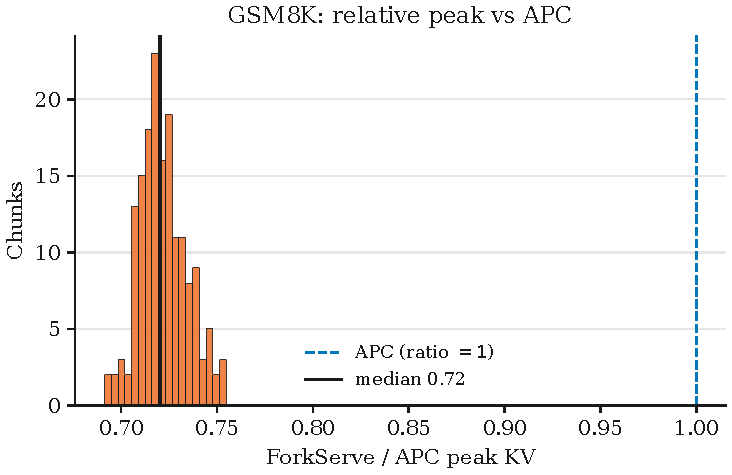
\includegraphics[width=\linewidth]{fig/peak_ratio_hist.pdf}
\end{minipage}
\caption{Left: aligned chunks, ForkServe vs.\ APC. All $165$ points lie below $y{=}x$. Right: ratio $\mathrm{peak}^{\mathrm{FS}}/\mathrm{peak}^{\mathrm{APC}}$, median $0.72$.}
\end{figure}

\begin{figure}[h]
\centering
\begin{minipage}{0.49\textwidth}
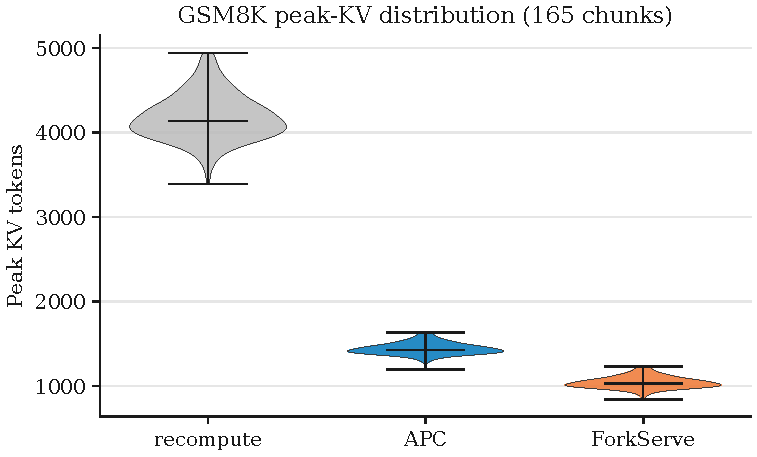
\includegraphics[width=\linewidth]{fig/peak_violin_gsm8k.pdf}
\end{minipage}\hfill
\begin{minipage}{0.49\textwidth}

\includegraphics[width=\linewidth]{fig/peak_median_gsm8k.pdf}
\end{minipage}
\caption{Left: the ForkServe--APC gap is a shift of the whole distribution, not a few outliers. Right: median $\mathrm{peak}$.}
\end{figure}

\begin{table}[h]
\centering
\small
\begin{tabular}{@{}lrrrrrr@{}}
\toprule
Serving & accuracy & med $\mathrm{peak}$ & max $\mathrm{peak}$ & p95 $\mathrm{peak}$ & med fan-out & generate \\
\midrule
recompute & 0.847 (1117) & 4136 & 4944 & --- & $326\,\mathrm{ms}$ & $19.4\,\mathrm{min}$ \\
APC       & 0.844 (1113) & 1430 & 1632 & 1572 & $87\,\mathrm{ms}$  & $18.6\,\mathrm{min}$ \\
ForkServe & \textbf{0.845 (1114)} & \textbf{1030} & \textbf{1232} & \textbf{1172} & $140\,\mathrm{ms}$ & $18.9\,\mathrm{min}$ \\
\bottomrule
\end{tabular}
\caption{GSM8K forest, $n{=}1319$, $k{=}4$, $\mathrm{tp}{=}2$.
Median $\mathrm{peak}^{\mathrm{FS}}/\mathrm{peak}^{\mathrm{APC}}{=}0.720$;
relative to recompute, $0.249$.}
\end{table}

Define the measured savings against the two baselines
\begin{equation}
\label{eq:save}
S_{\mathrm{APC}}
  = 1-\frac{\mathrm{med}(\mathrm{peak}^{\mathrm{FS}})}{\mathrm{med}(\mathrm{peak}^{\mathrm{APC}})}
  \approx 28\%,
\qquad
S_{\mathrm{clone}}
  = 1-\frac{\mathrm{med}(\mathrm{peak}^{\mathrm{FS}})}{\mathrm{med}(\mathrm{peak}^{\mathrm{rec}})}
  \approx 75\%.
\end{equation}
$S_{\mathrm{clone}}$ is the $k{\approx}4$ clone regime: four thoughts pay four trunks under recompute and one under CoW.
$S_{\mathrm{APC}}{>}0$ is not implied by prefix caching alone.
APC already avoids most of $M_{\mathrm{clone}}$ (median $1430$ vs.\ $4136$).
ForkServe still reduces the remainder because abort frees loser residuals immediately, and the spine is not the union of hashed sibling prefixes.
The scatter plot is $\forall\,\mathrm{chunks}:\;\mathrm{peak}^{\mathrm{FS}}<\mathrm{peak}^{\mathrm{APC}}$.

\subsection{Quality}

\begin{figure}[h]
\centering

\includegraphics[width=\textwidth]{fig/accuracy_running_gsm8k.pdf}
\caption{\label{fig:acc}Official GSM8K extractor, running accuracy. Forest accuracy ($\approx 0.845$) is below single-path quality-only ($\approx 0.941$) because the recipe is ToT, not a unique continuation. Recompute, APC, and ForkServe stay aligned.}
\end{figure}

Running accuracy of recompute, APC, and ForkServe stays in $[0.83,0.85]$ (Figure~\ref{fig:acc}); terminal counts differ by $1$--$3$ items.

\subsection{Fan-out time and e2e}

On this ToT path the four thoughts are known residuals.
Median fan-out per chunk is $326\,\mathrm{ms}$ (recompute), $87\,\mathrm{ms}$ (APC), $140\,\mathrm{ms}$ (ForkServe):
\begin{equation}
T_{\mathrm{fan}}^{\mathrm{rec}}
  \;\approx\;
  k\cdot T_{\mathrm{pre}}(L+\bar\ell),
\qquad
T_{\mathrm{fan}}^{\mathrm{APC}}
  \;\approx\;
  T_{\mathrm{pre}}(L)+k\cdot T_{\mathrm{pre}}(\bar\ell).
\end{equation}
ForkServe pays $T_{\mathrm{pre}}(L)$ once at open and $k\cdot T_{\mathrm{pre}}(\bar\ell)$ as CoW residuals.
APC is still the fastest fan-out ($87$ vs.\ $140\,\mathrm{ms}$).
E2e is dominated by winner decode of $512$ tokens: APC records $T_{\mathrm{decode}}{\approx}1075\,\mathrm{s}$ of $T_{\mathrm{e2e}}{\approx}1102\,\mathrm{s}$, fan-out $14\,\mathrm{s}$.
A $1.61\times$ fan-out gap is second-order in $T_{\mathrm{e2e}}$.

\begin{figure}[h]
\centering

\includegraphics[width=\textwidth]{fig/fanout_trace_gsm8k.pdf}
\caption{Per-chunk fan-out. APC is fastest; ForkServe is slower than APC but far below recompute.}
\end{figure}

\begin{figure}[h]
\centering
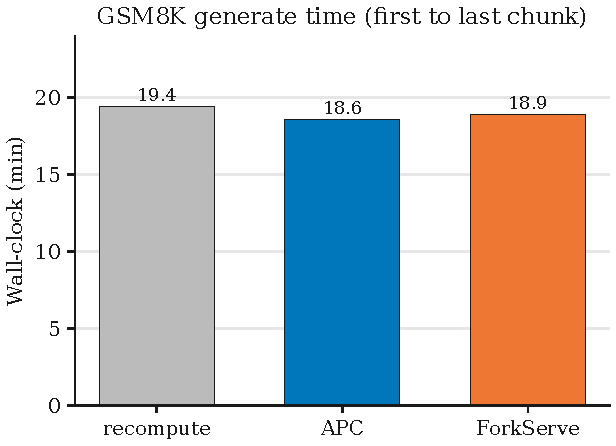
\includegraphics[width=0.62\textwidth]{fig/generate_wallclock_gsm8k.pdf}
\caption{Generate wall-clock. ForkServe is $+0.3\,\mathrm{min}$ vs.\ APC ($+1.6\%$).}
\end{figure}

The GSM8K run evaluates fork and abort on committed ToT thoughts, not speculative observation guesses.

\section{Small forest: GSM8K, Game24, HumanEval ($n=4$)}

RL round~3 runs the same forest with $n{=}4$ items, $\mathrm{tp}\in\{2,4\}$, and enough decode for the winner to finish.
We report pairs with $\mathrm{peak}^{\mathrm{FS}}<\mathrm{peak}^{\mathrm{APC}}$ and no official-score drop vs.\ APC.
(The $\mathrm{tp}{=}4$ GSM8K pair is omitted: APC $1.00$ vs.\ ForkServe $0.75$ on four items; the $n{=}1319$ result supersedes it.)

\begin{figure}[h]
\centering
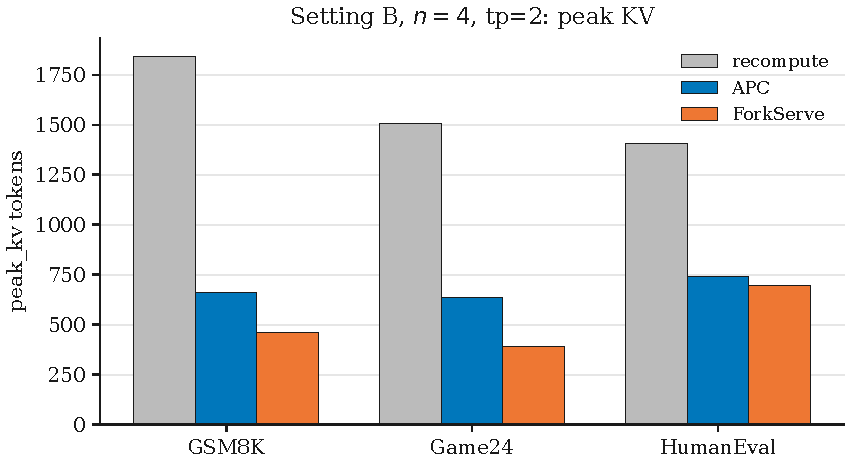
\includegraphics[width=0.92\textwidth]{fig/rl3_peak_tp2.pdf}
\caption{$\mathrm{tp}{=}2$, $n{=}4$: $\mathrm{peak}$. GSM8K $459{<}659$, Game24 $390{<}638$, HumanEval $695{<}739$.}
\end{figure}

\begin{figure}[h]
\centering

\includegraphics[width=0.92\textwidth]{fig/rl3_lat_tp2.pdf}
\caption{$\mathrm{tp}{=}2$ e2e vs.\ APC: $-0.3\%$, $-0.7\%$, $+0.1\%$.}
\end{figure}

\begin{table}[h]
\centering
\small
\begin{tabular}{@{}llcccc@{}}
\toprule
tp & recipe & $\mathrm{peak}^{\mathrm{FS}}$ & $\mathrm{peak}^{\mathrm{APC}}$ & ratio & official (FS $=$ APC) \\
\midrule
2 & ToT / GSM8K     & 459 & 659 & $0.70$ & acc.\ $0.75$ \\
2 & ToT / Game24    & 390 & 638 & $0.61$ & success $1.00$ \\
2 & ReAct / HumanEval & 695 & 739 & $0.94$ & pass@1 $0.75$ \\
4 & ToT / Game24    & 390 & 638 & $0.61$ & success $1.00$ \\
4 & ReAct / HumanEval & 695 & 739 & $0.94$ & pass@1 $0.75$ \\
\bottomrule
\end{tabular}
\caption{RL round~3, completed pairs with efficiency beat and no quality drop. HumanEval latency is judged on TTFT from observation; e2e gaps remain ${<}2\%$. $\mathrm{peak}$ is independent of $\mathrm{tp}$ here: it counts tokens, not sharded bytes.}
\end{table}

\begin{figure}[h]
\centering
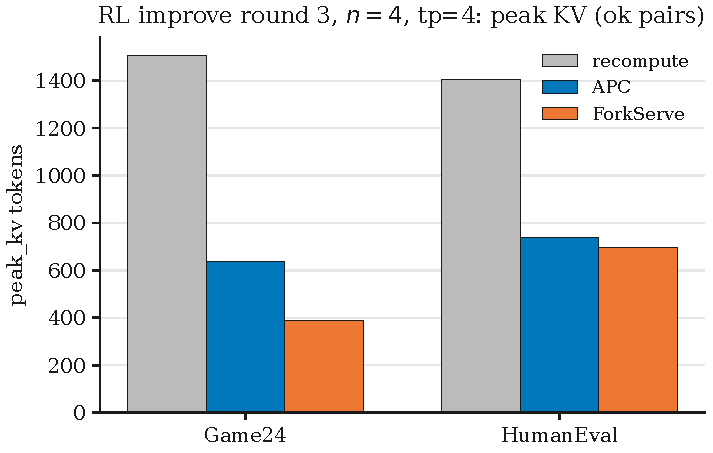
\includegraphics[width=0.72\textwidth]{fig/rl3_peak_tp4_ok.pdf}
\caption{$\mathrm{tp}{=}4$ ToT Game24 and ReAct HumanEval: same spine vs.\ APC gap as $\mathrm{tp}{=}2$.}
\end{figure}

\paragraph{Ratios.}
ToT ($k{=}4$) gives $\mathrm{peak}^{\mathrm{FS}}/\mathrm{peak}^{\mathrm{APC}}\in[0.61,0.70]$.
ReAct ($k{=}2$) gives $0.94$: residuals are large relative to $L$, so the spine cannot approach $1/k$.
Full-set GSM8K ($0.72$) matches $n{=}4$ GSM8K ($0.70$).
HumanEval wrap+recovery are known suffixes; committed-path e2e/TTFT did not regress while $\mathrm{peak}$ fell.

\section{Discussion}
{\sloppy
APC already removes most trunk recompute.
The remaining HBM cost of a fan-out is whether unused siblings stay resident.
Prefix caching shares after a hash hit; ForkServe shares at fork and drops losers at abort.
GSM8K $n{=}1319$ shows the latter is leaner in $\mathrm{peak}$ and interchangeable in accuracy and e2e.
Fan-out is still slower than APC.
$n{=}4$ quality is a sanity check; the $1319$-item extractor is the quality claim.
}

\section{Conclusion}

On Qwen3-14B, $\mathrm{tp}{=}2$, ToT forest, GSM8K test:
\begin{equation}
\mathrm{peak}^{\mathrm{FS}}
  = 0.72\cdot\mathrm{peak}^{\mathrm{APC}}
  = 0.25\cdot\mathrm{peak}^{\mathrm{rec}},
\quad
\mathrm{acc}^{\mathrm{FS}}
  \approx \mathrm{acc}^{\mathrm{APC}},
\quad
\frac{T_{\mathrm{e2e}}^{\mathrm{FS}}}{T_{\mathrm{e2e}}^{\mathrm{APC}}}
  \approx 1.016.
\end{equation}
The $n{=}4$ forest reproduces the $\mathrm{peak}$ ordering on ToT and ReAct, including $\mathrm{tp}{=}4$ Game24 and HumanEval.

\end{document}
